\documentclass[11pt]{article}
\usepackage{geometry,marginnote} % Pour passer au format A4
\geometry{hmargin=1cm, vmargin=1.5cm} % 

% Page et encodage
\usepackage[T1]{fontenc} % Use 8-bit encoding that has 256 glyphs
\usepackage[english,french]{babel} % Français et anglais
\usepackage[utf8]{inputenc} 

\usepackage{lmodern}
\usepackage[np]{numprint}
\setlength\parindent{0pt}

% Graphiques
\usepackage{graphicx,float,grffile}
\usepackage{tikz,pst-eucl,pst-plot,pstricks,pst-node,pstricks-add,pst-fun,pgfplots} 

% Maths et divers
\usepackage{amsmath,amsfonts,amssymb,amsthm,verbatim,scratch3}
\usepackage{multicol,enumitem,url,eurosym,gensymb,tabularx}

\DeclareUnicodeCharacter{20AC}{\euro}



% Sections
\usepackage{sectsty} % Allows customizing section commands
\allsectionsfont{\centering \normalfont\scshape}

% Tête et pied de page
\usepackage{fancyhdr} \pagestyle{fancy} \fancyhead{} \fancyfoot{}

%\fancyfoot[L]{Collège Faubert}
%\fancyfoot[C]{\thepage / 6}
%\fancyfoot[R]{Série Générale}

\renewcommand{\headrulewidth}{0pt} % Remove header underlines
%\renewcommand{\footrulewidth}{0pt} % Remove footer underlines

\newcommand{\horrule}[1]{\rule{\linewidth}{#1}} % Create horizontal rule command with 1 argument of height

\newcommand{\Pointilles}[1][3]{%
  \multido{}{#1}{\makebox[\linewidth]{\dotfill}\\[\parskip]
}}

\newtheorem{Definition}{Définition}

\usepackage{siunitx}
\sisetup{
    detect-all,
    output-decimal-marker={,},
    group-minimum-digits = 3,
    group-separator={~},
    number-unit-separator={~},
    inter-unit-product={~}
}

\setlength{\columnseprule}{1pt}



\begin{document}

{\Large \textsc{Devoir Commun - Mathématiques}}

\begin{itemize}
    \item L'usage de la calculatrice de type collège est autorisé. L'usage de tout autre document est interdit. 
    \item L'ensemble des réponses pour les exercices 2 et 3 devront êtres justifiées.
    \item Toute trace écrite, même incomplète sera prise en compte dans l'évaluation.
  \end{itemize}

\horrule{2px}

\subsection*{Exercice 1 - 12 points}

\begin{multicols}{2}

    \begin{enumerate}
        \item[1.] La valeur de l’angle manquant est :
        \begin{figure}[H]
            \centering
            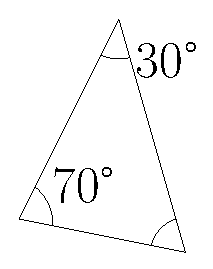
\includegraphics[width=0.2\linewidth]{qcm1.eps}
        \end{figure}

        \item[2.] Voici une série de valeur : 18 ; 9 ; 12. \newline 
        La moyenne de cette série est : 

        \item[3.] On lance la roue équilibrée suivante : \newline 
        Les 8 emplacements sont identiques.
        \begin{figure}[H]
            \centering
            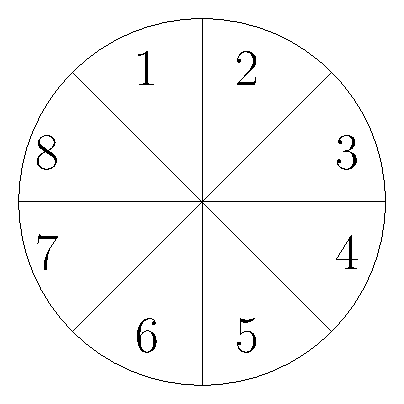
\includegraphics[width=0.2\linewidth]{qcm3.eps}
        \end{figure}
        Quelle est la probabilité de tomber sur un nombre pair ? 
        \item[4.] $\left( \dfrac{2}{3} - \dfrac{1}{3} \times \dfrac{7}{5} \right) \div \dfrac{4}{3} = $
    \end{enumerate} \columnbreak
    
    \begin{itemize}[label={$\bullet$}]
        \item Il faut répondre sur la copie. 
        \item Une seule réponse juste.
        \item Aucune justification demandée pour le QCM.
    \end{itemize}

    \begin{center} \begin{tabular}{|c|c|c|c|c|}  \hline
        & A & B & C & D \\ \hline
        1. $\phantom{\dfrac{\dfrac{1}{1}}{\dfrac{1}{1}}}$  & 70° & 80° & 180° & 100° \\ \hline
        2. $\phantom{\dfrac{\dfrac{1}{1}}{\dfrac{1}{1}}}$  &   9 &  12 &   13 & 31   \\ \hline
        3. $\phantom{\dfrac{\dfrac{1}{1}}{\dfrac{1}{1}}}$  & $\dfrac{1}{8}$ & $\dfrac{1}{2}$ & $\dfrac{3}{8}$ & $\dfrac{1}{4} $ \\ \hline
        4. $\phantom{\dfrac{\dfrac{1}{1}}{\dfrac{1}{1}}}$  & $\dfrac{3}{15} \times \dfrac{4}{3}$ & $\left(\dfrac{1}{3} \times \dfrac{7}{5} \right) \div \dfrac{4}{3}$ & $\dfrac{3}{15} \times \dfrac{3}{4}$ & $\dfrac{7}{5} \times \dfrac{3}{4} $  \\ \hline
    \end{tabular} \end{center}

\end{multicols}

\subsection*{Exercice 2 - 20 points}

Michel participe à un rallye VTT sur un parcours balisé. Le trajet est représenté en traits pleins.

Le départ du rallye est en A et l'arrivée est en G.

\begin{multicols}{2}
    \medskip

    \begin{itemize}[label={$\bullet$}]
        \item Le dessin n'est pas à l'échelle.
        \item Les points A, B et C sont alignés.
        \item Les points C, D et E sont alignés.
        \item Les points B, D et F sont alignés.
        \item Les points E, F et G sont alignés.
        \item Le triangle BCD est rectangle en C.
        \item Le triangle DEF est rectangle en E.
    \end{itemize}

    \medskip

    \begin{enumerate}
        \item[1.] Montrer que la longueur BD est égale à $2,5$~km.

        \item[2.] Justifier que les droites (BC) et (EF) sont parallèles.

        \item[3.] Calculer la longueur DF.

        \item[4.] Calculer la longueur totale du parcours.

        \item[5.] Michel roule à une vitesse moyenne de $16$~km/h pour aller du point A au point B.

        Combien de temps mettra-t-il pour aller du point A au point B ?

        Donner votre réponse en minutes et secondes. 
    \end{enumerate} \columnbreak

    \begin{center}
    \psset{unit=0.85cm}
    \begin{pspicture}(10,8)
    %\psgrid
    \psline[linewidth=1.25pt](0.5,7.5)(4.5,7.5)(9,0.5)(11,0.5)%AB(D)FG
    \uput[u](0.5,7.5){A} \uput[u](4.3,7.5){B}\uput[u](6.5,7.5){C}
    \uput[ur](6,5){D}\uput[d](6,0.5){E}\uput[d](9,0.5){F}
    \uput[d](11,0.5){G}
    \psline[linestyle=dashed,linewidth=1.25pt](4.5,7.5)(6,7.5)(6,0.5)(9,0.5)%BCEF
    \uput[u](5.25,7.5){1,5 km}\uput[u](2.5,7.5){7 km}
    \uput[r](6,6.25){2 km}\uput[l](6,2.75){5 km}\uput[d](10,0.5){3,5 km}
    \end{pspicture}
    \end{center}
\end{multicols}

\subsection*{Exercice 3 - 18 points}

\medskip

\begin{minipage}[t]{0.5\textwidth}
    \begin{enumerate}
        \item[1.] On considère le programme A défini par le schéma ci-contre :
        \begin{enumerate}
            \item[1a.] Vérifier que le résultat est $60$ si le nombre choisi au départ est $-8$.
            \item[1b.] On appelle $x$ le nombre de départ. \newline
            Prouver que le résultat de ce programme de calcul peut s’écrire sous la forme $x^2 - x - 12$.
        \end{enumerate}
    \end{enumerate}
\end{minipage}\hfill
\begin{minipage}[t]{0.5\textwidth}
    \begin{center}
    \psset{unit=1cm,arrowsize=2pt 3}
    \begin{pspicture}(-3.8,0)(3.8,7.4)
    %\psgrid
    \psframe(-0.9,5.4)(0.9,6.2)\psframe(-0.9,0)(0.9,0.8)
    \psframe(-3.8,3.1)(-2,3.9)\psframe(3.8,3.1)(2,3.9)
    \rput(-2.3,4.8){Ajouter 3}\rput(2.7,4.8){Soustraire 4}
    \rput(0,7.1){Choisir un nombre}
    \rput(0,2.7){Multiplier les deux}\rput(0,2.2){résultats}
    \psline{->}(0,6.9)(0,6.2)\psline{->}(0,5.4)(-2.9,3.9)\psline{->}(0,5.4)(2.9,3.9)
    \psline(-2.9,3.1)(0,1.4)\psline(2.9,3.1)(0,1.4)
    \psline{->}(0,1.4)(0,0.8)
    \end{pspicture}
    \end{center}
\end{minipage}

\begin{minipage}[t]{0.4\textwidth}
\begin{enumerate}[resume]
    \item[2.] On rappelle que $x$ désigne le nombre de départ du programme de calcul. \newline
    On appelle f la fonction qui, à x, associe le résultat du programme de calcul. \newline
    On rappelle que $f(x) = x^2 - x - 12$. \\

    Calculer $f\left(\dfrac{1}{2}\right)$.

    \item[3.] Déterminer graphiquement les valeurs exactes des antécédents de 0 par la fonction $f$. \newline
    Aucune justification n’est attendue.
    
    \item[4.] Vérifier par le calcul que les valeurs trouvées par lecture graphique à la question précédente sont bien les antécédents de $0$ par la fonction $f$.
\end{enumerate}  
\end{minipage}\hfill
\begin{minipage}[t]{0.6\textwidth}
    \begin{center}
        \psset{xunit=0.7cm,yunit=0.4cm,arrowsize=2pt 3}
        \begin{pspicture*}(-5,-13)(6,12)
        \psaxes[linewidth=1.25pt,labelFontSize=\scriptstyle]{->}(0,0)(-4.99,-12.99)(6,12)
        \psplot[plotpoints=2000,linewidth=1.25pt,linecolor=blue]{-5}{6}{x dup mul x sub 12 sub}
        \uput[l](-4.2,10){\blue $\mathcal{C}_f$}
        \end{pspicture*}
        \end{center}
    \end{minipage}
\end{document}
